\begin{adjustbox}{width=.95\paperwidth, center}
	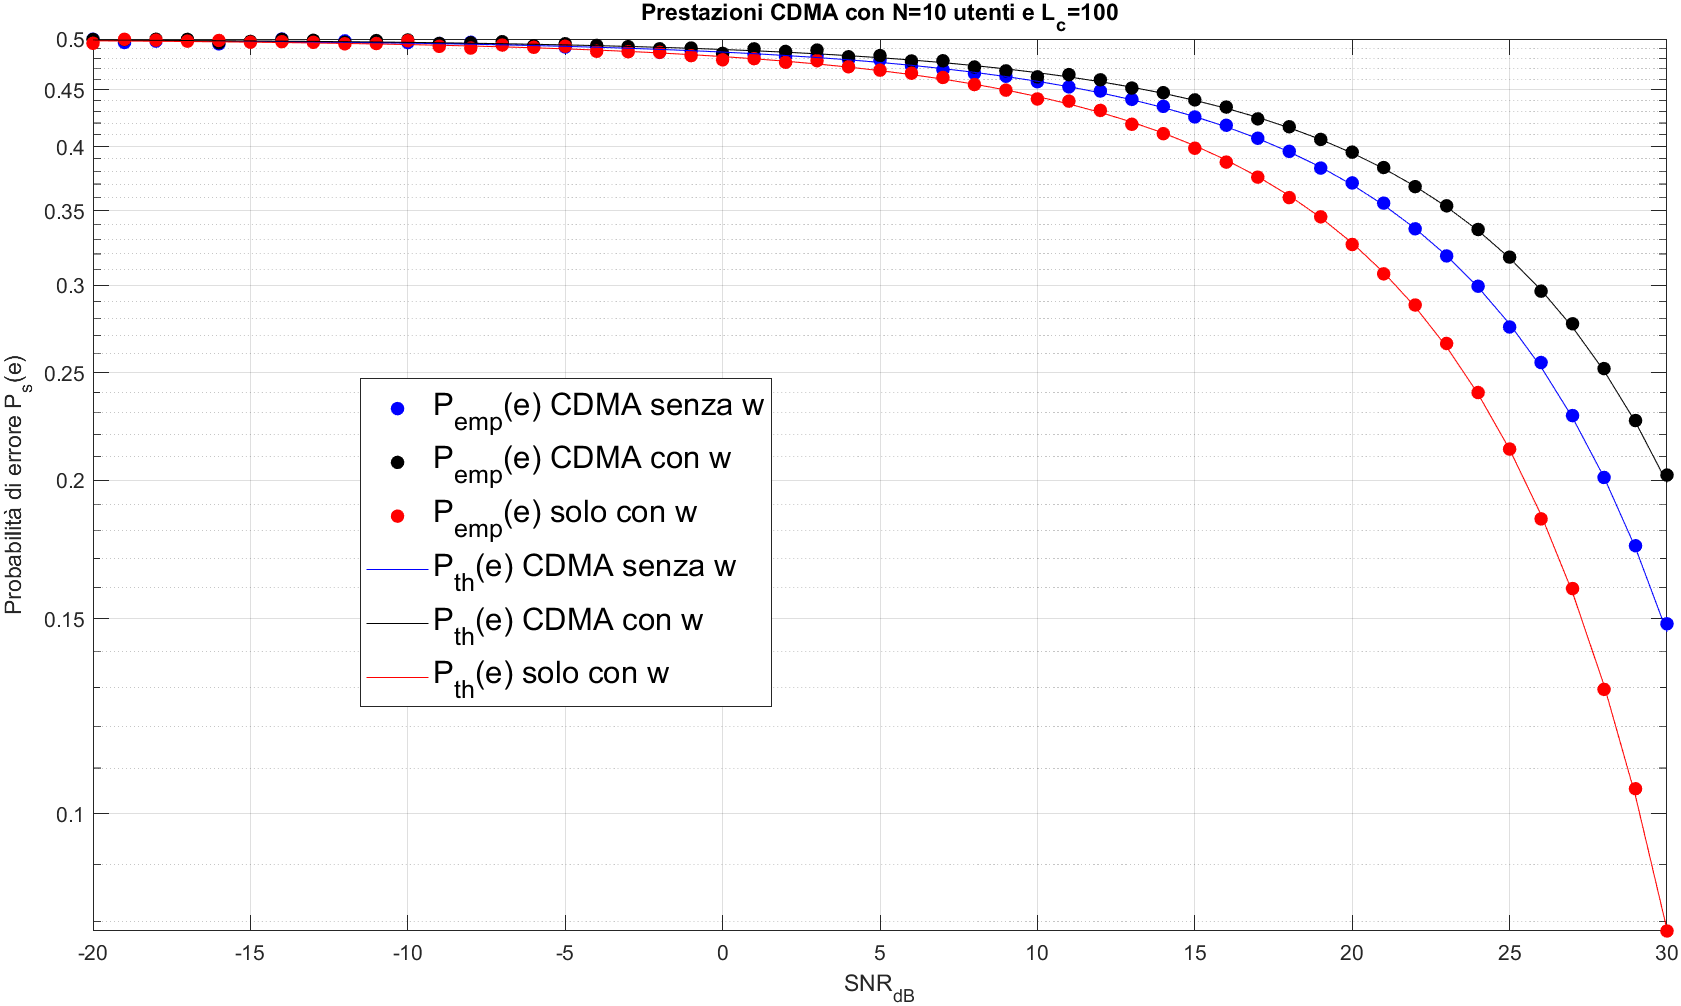
\includegraphics{images/prestazioniCDMA1.png}
\end{adjustbox}\\\\
Simulando la trasmissione CDMA con \(N=10\) e \(L_c=100\) sono state ricavate le tre \(P_{emp}(e)\) e le rispettive \(P_{th}(e)\) che seguono lo stesso andamento.\vspace{.3cm}\\
La \(P_{emp}(e)\) blu rappresenta le prestazioni della trasmissione CDMA senza rumore \(w\) aggiuntivo, considerando quindi \(s_1 = \mathcal{E}_s \pm n, \; n\sim\mathcal{N}(0,\,L_c(N-1))\).\vspace{.3cm}\\
La \(P_{emp}(e)\) nera rappresenta le prestazioni della trasmissione CDMA con rumore \(w\) aggiuntivo,\\
considerando quindi \(s_1 = \mathcal{E}_s \pm n + w, \; w\sim\mathcal{N}(0,\,\frac{N_0}{2})\).\vspace{.3cm}\\
La \(P_{emp}(e)\) rossa rappresenta le prestazioni della trasmissione con solo rumore \(w\),\\ considerando quindi \(s_1 = \mathcal{E}_s + w\).\vspace{.3cm}\\
Si nota dal grafico che la \(P(e)\) nera decade più lentamente rispetto alle altre al crescere di \(SNR_{dB}\) e denota quindi le prestazioni peggiori.\\
In questa simulazione è stato scelto \(N_0\) di \(w\) tale da non influire eccessivamente nella trasmissione per ottenere tre andamenti distinti. Infatti se si aumentasse \(N_0\), la \(P(e)\) nera si sovrapporrebbe con la \(P(e)\) rossa perchè il rumore \(n\) risulterebbe trascurabile rispetto a \(w\), mentre la \(P(e)\) blu denoterebbe le prestazioni migliori.